\documentclass[aspectratio=169]{beamer}
\setbeamertemplate{footline}[frame number]
%\documentclass[aspectratio=169,notes=only]{beamer}
\usepackage{multicol}
\usepackage{wrapfig}
\usepackage{algorithmicx}
\usepackage{algpseudocode}
\usepackage{graphicx}
%\usepackage{subcaption} % cannot be used

\usepackage[english]{layout}
\usepackage[utf8]{inputenc}
\usepackage[english]{babel}
\usepackage[T1]{fontenc}
\usepackage{amsmath, soul, color, multicol, type1cm, verbatim, latexsym, dsfont, float, listings,alltt,tikz, lmodern, textcomp}
\usepackage[official]{eurosym}
\usepackage[export]{adjustbox}
\usepackage[caption = false]{subfig}
%\usepackage{beamerthemesplit}
%\usetheme{Frankfurt}
\usecolortheme{lily}
%\usefonttheme{structuresmallcapsserif}
\usefonttheme{professionalfonts}
\setbeamercovered{transparent}

\newcommand{\pluseq}{\mathrel{{+}{=}}}

%NeSI Colors <-------------------------------------------------------------------------------------
\usecolortheme{lily}
\usecolortheme[RGB={47, 68, 71}]{structure} 
\definecolor{nesidark}{HTML}{2F4447}
\definecolor{nesilight}{HTML}{CED9DF}
\definecolor{nesigrey}{gray}{0.7}
\definecolor{nesilightgrey}{gray}{0.98}
\definecolor{nesidarkgrey}{gray}{0.3}
\definecolor{nesiblue}{HTML}{2B9FC2}
\setbeamercolor{block title}{fg=black,bg=nesigrey}
\setbeamercolor{block body}{bg=nesilightgrey,fg=nesidarkgrey}
\setbeamercolor{block body alerted}{bg=white,fg=black}
\setbeamercolor{alerted text}{bg=white,fg=black}
\addtobeamertemplate{frametitle}{\vskip+1.2ex}{}
%NeSI Custom Code Hightlight <---------------------------------------------------------------------------------------
\lstdefinestyle{customcode}{
  belowcaptionskip=1\baselineskip,
  breaklines=true,
  xleftmargin=\parindent,
  showstringspaces=false,
  basicstyle=\ttfamily,
  keywordstyle=\bfseries\color{green!40!black},
  commentstyle=\itshape\color{purple!40!black},
  identifierstyle=\color{blue},
  stringstyle=\color{orange},
}
%NeSI Title <---------------------------------------------------------------------------------------
\setbeamerfont{title}{size=\huge}
\frenchspacing
\hyphenation{NeSI}
%NeSI Template parameters <-------------------------------------------------------------------------
\setbeamertemplate{blocks}[default]
\useinnertheme{circles}
\setbeamertemplate{title page}[default][center,rounded=false,shadow=false]
\newcommand\BackgroundPicture[1]{%
\setbeamertemplate{background}{%
\parbox[c][\paperheight]{\paperwidth}{%
\vfill \hfill \includegraphics[height=\paperheight]{#1}
\hfill \vfill
}}}

%\pagenumbering{arabic}

%Content Starts Here <-------------------------------------------------------------------------------
\title{\LARGE{Two interpolation methods for vector fields that conseve flux and line integrals}}
%\subtitle{Computational Science team}
\author{Alexander Pletzer (NeSI/NIWA) and Wolfgang Hayek (NIWA/NeSI)\\
(alexander.pletzer@nesi.org.nz) \\
 C3DIS, Canberra\\
 7 May 2019  }
\date{}

\begin{document}
\BackgroundPicture{NeSI/title.png}
\begin{frame}[plain]
  \vspace{+1.0cm}
  \titlepage
\end{frame}

% This will generate the outline. If you have several topics, uncomment the multicols 
\BackgroundPicture{NeSI/blank-01.png}

%%%%%%%%%%%%%%%%%%%%%%%%%%%%%%%%%%%%%%%%%%%%%%%%%%%%%%%%%%%%%%%%%%%%%%%%%%%%%%%%%%%%%%%%%%%%%%%
%%%%%%%%%%%%%%%%%%%%%%%%%%%%%%%%%%%%%%%% Some Examples %%%%%%%%%%%%%%%%%%%%%%%%%%%%%%%%%%%%%%%%
%%%%%%%%%%%%%%%%%%%%%%%%%%%%%%%%%%%%%%%%%%%%%%%%%%%%%%%%%%%%%%%%%%%%%%%%%%%%%%%%%%%%%%%%%%%%%%%
% List with bullets (itemize) <---
% The [<+-| alert@+>] will create a new slide for each element with highlighting 


\begin{frame}[t]
  \frametitle{Motivation: want answers to:}
    \begin{block}{How to interpolate vector fields with staggered components?}
      \begin{itemize}%[<+-| alert@+>]
	  \item Arakawa C/D grids
      \item Components are on cell faces or edges
      \item Arises in computational fluid dynamics and electromagnetics
    \end{itemize}
  \end{block}
  \begin{tabular}{lr}
      % after \\: \hline or \cline{col1-col2} \cline{col3-col4} ...
      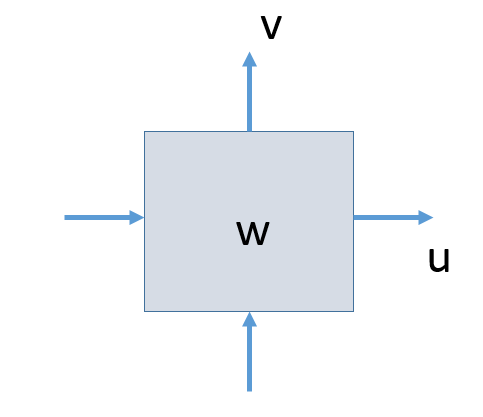
\includegraphics[width=30mm]{uvArakawaC.PNG} &               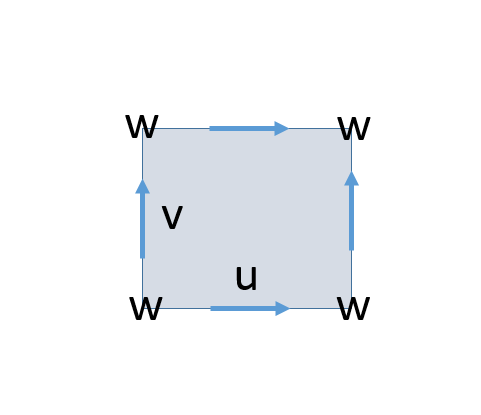
\includegraphics[width=30mm]{uvArakawaD.PNG} \\
      {Arakawa C-grid} & {Arakawa D-grid}  
\end{tabular}
\end{frame}

\begin{frame}[t]
  \frametitle{Currently used interpolation methods in earth sciences}
    \begin{block}{Is there hope to unify these?}
      \begin{itemize}%[<+-| alert@+>]
	  \item Linear, used since Babylonian times (2000-1700 BC)
      \item Conservative or area weighted, used in climate studies to enforce conservation of total mass, energy
    \end{itemize}
  \end{block}
  \begin{tabular}{lr}
      % after \\: \hline or \cline{col1-col2} \cline{col3-col4} ...
      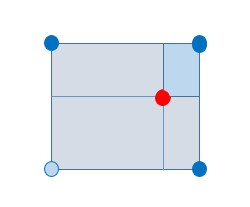
\includegraphics[width=30mm]{bilinear.png} &               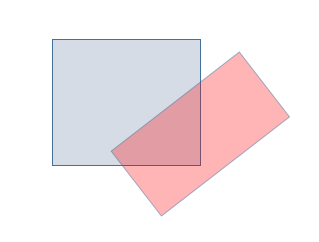
\includegraphics[width=30mm]{conservative.png} \\
      {Bilinear} & {Conservative}  
\end{tabular}
\end{frame}

\begin{frame}[t]
  \frametitle{Earth science grids are curvilinear}
  \begin{block}{How to handle non-orthogonal cells?}
    Example: cubed-sphere grid
    \begin{itemize}
      \item Project grids on the surface of a cube onto a sphere
      \item Six logically rectangular grids (cannot be represented as a single structured grid)
      \item No pole-like singularity but some distortion where three tiles meet 
    \end{itemize}
  \end{block}
  \begin{center}
    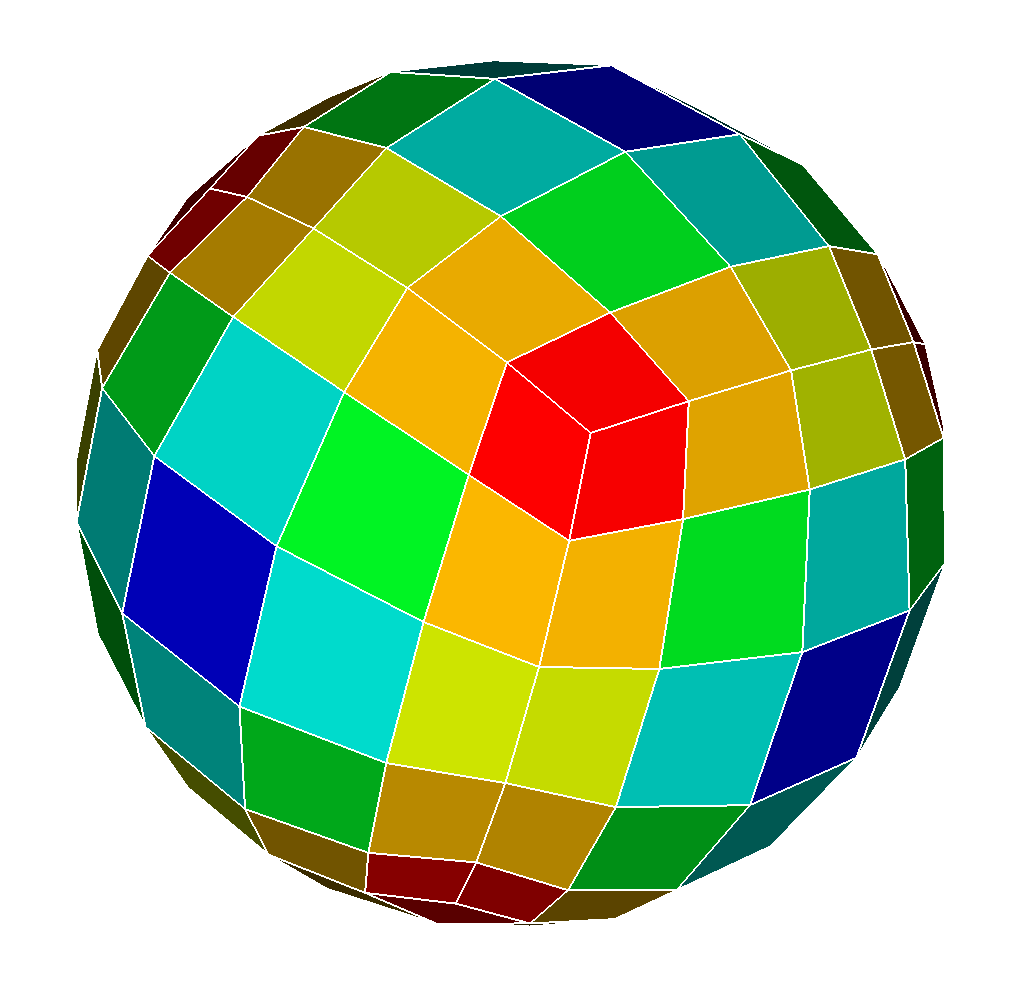
\includegraphics[width=0.35\textwidth]{cubedSphere.png}
  \end{center}
\end{frame}

\begin{frame}[t]
  \frametitle{Interpolation is needed to:}
  \begin{itemize}
   \item compute fluxes across area
   \item advect fields
   \item determine statistical properties in given regions
  \end{itemize}
  \begin{center}
    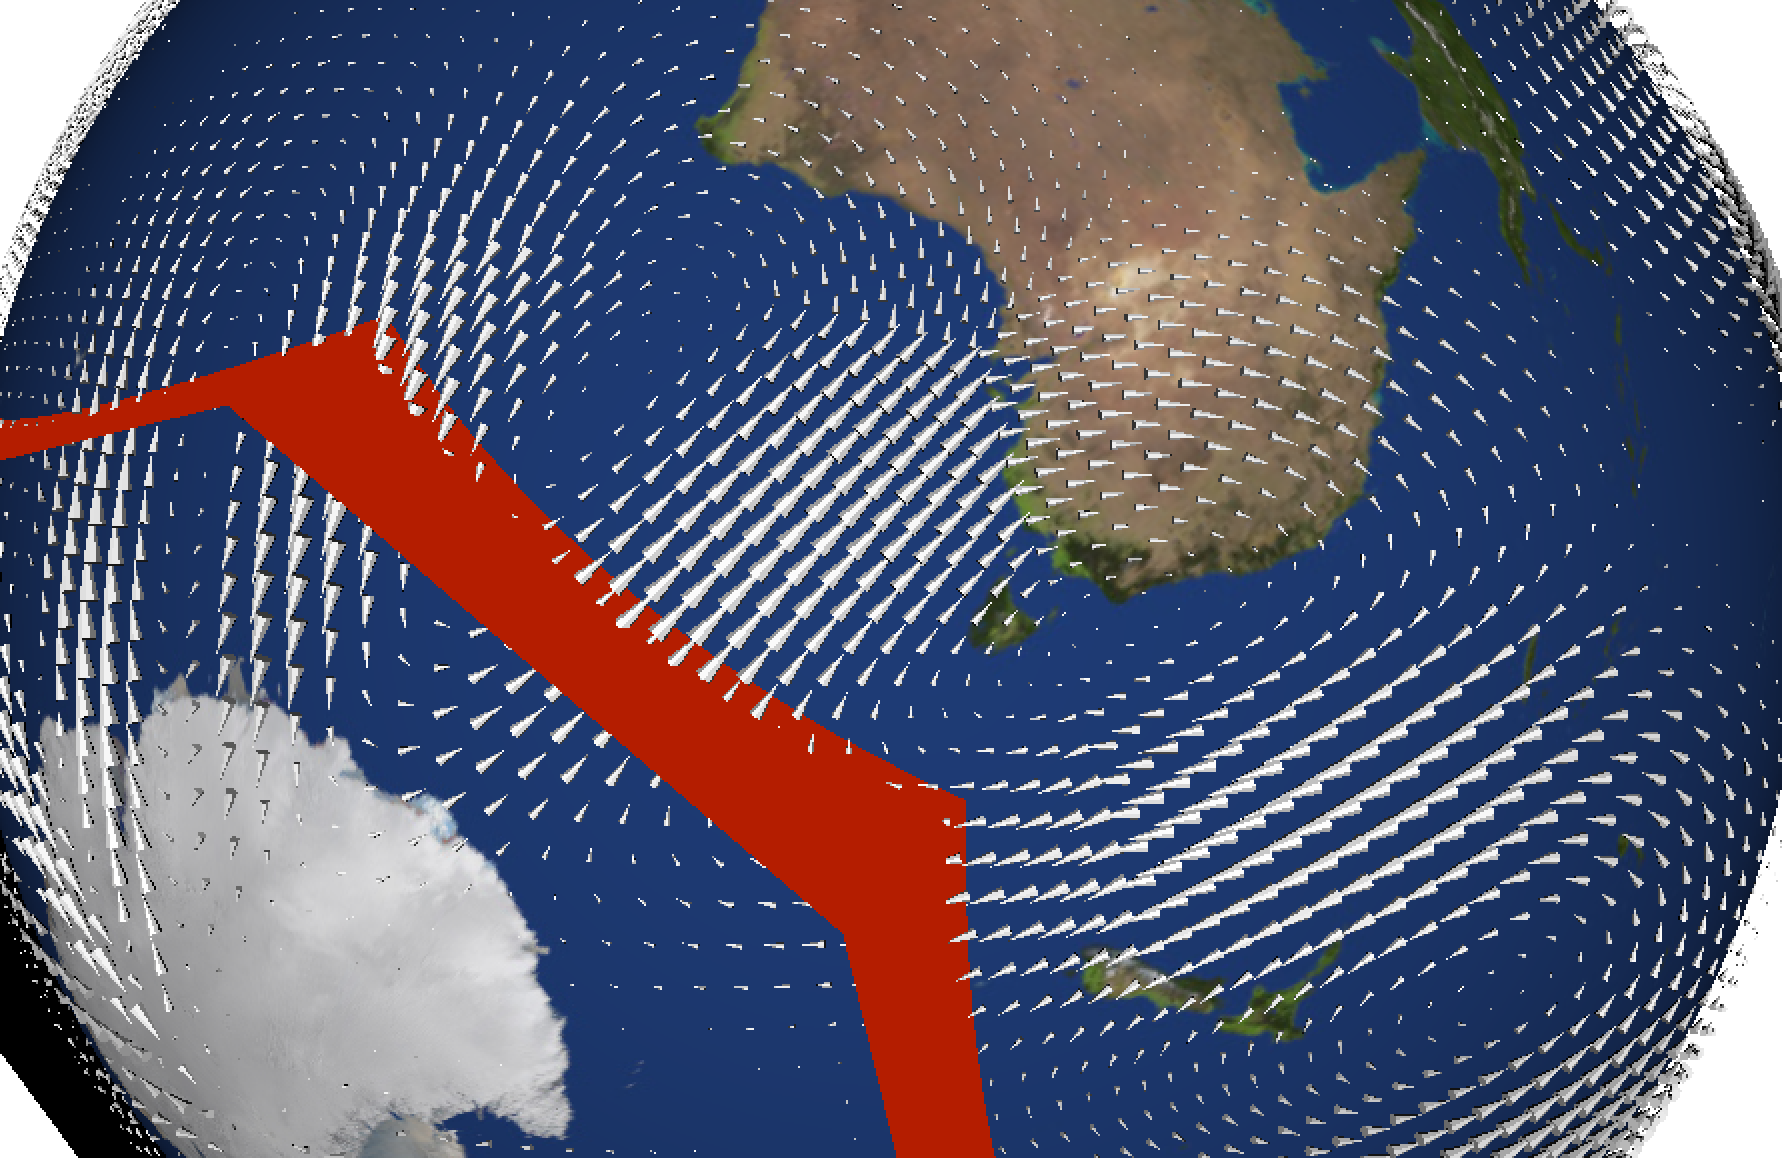
\includegraphics[width=0.6\textwidth]{fluxIntegral.png}
  \end{center}
  
\end{frame}

\begin{frame}[t]
  \frametitle{Four types of fields - one derivative}
    \begin{block}{Exterior calculus tells us:}
      \begin{itemize}%[<+-| alert@+>]
	  \item {\color{red} 0-form}: just a function of space, one component
        \begin{itemize}
          \item invariant under coordinate change
          \item Example: temperature
        \end{itemize}
      \item {\color{red} 1-form}: vector field, 3 components in 3D
        \begin{itemize}
          \item Examples: electric field $E$, induction $H$ and velocity
        \end{itemize}
      \item {\color{red} 2-form}: pseudo-vector field, 3 components in 3D
         \begin{itemize}
          \item Examples: magnetic field $B$, displacement field $D$ and vorticity
        \end{itemize}
   \item {\color{red} 3-form}: pseudo-scalar, 1 component
         \begin{itemize}
          \item Example: density
        \end{itemize}
    \end{itemize}
  \end{block}
\end{frame}

\begin{frame}[t]
  \frametitle{Discretized fields corresponding to the 1-3 forms}
    \begin{block}{Association of form with cell elements}
      \begin{itemize}%[<+-| alert@+>]
	  \item 0-form: {\color{red} on nodes}
        \begin{itemize}
          \item $\int \alpha = \alpha$ (integral is a no op)
        \end{itemize}
      \item 1-form: {\color{red} on edges}
        \begin{itemize}
          \item $\int \beta$ is a line integral
        \end{itemize}
      \item 2-form: {\color{red} on faces}
        \begin{itemize}
          \item $\int \gamma$ is a surface integral
        \end{itemize}
      \item 3-form: {\color{red} cell centred}
        \begin{itemize}
          \item $\int \omega$ is a volume integral
        \end{itemize}
    \end{itemize}
  \end{block}
  \begin{block}{Differential forms like to be integrated}
  \end{block}
\end{frame}

\begin{frame}[fragile]{Generalizing ``interpolation''}
\begin{block}{Making interpolation work for nodal, edge, face and cell fields}
$\int f = \sum_i f_i \int_T \phi_i$
\begin{itemize}
\item $\phi_i$ is basis $k$-form, $k =$ 0, 1, 2 or 3
\item $T$ is target (point, line, area or volume)
\item $f_i$ is field integral over cell element $k$ (node, edge, face or cell)
\item $\int_T \phi_i$ is the {\color{red} interpolation weight}
\item $i$ index runs over all the degrees of freedom (points, edges, faces etc., as appropriate)
\end{itemize}
\end{block}
\end{frame}

\begin{frame}[fragile]{Basis functions satisfy orthogonality condition}

\begin{block}{$\int_i \phi_j = \delta_{ij}$}
   $i$ is cell element (node, edge, face, cell), $j$ is basis function index
 \end{block}
  \begin{tabular}{lr}
      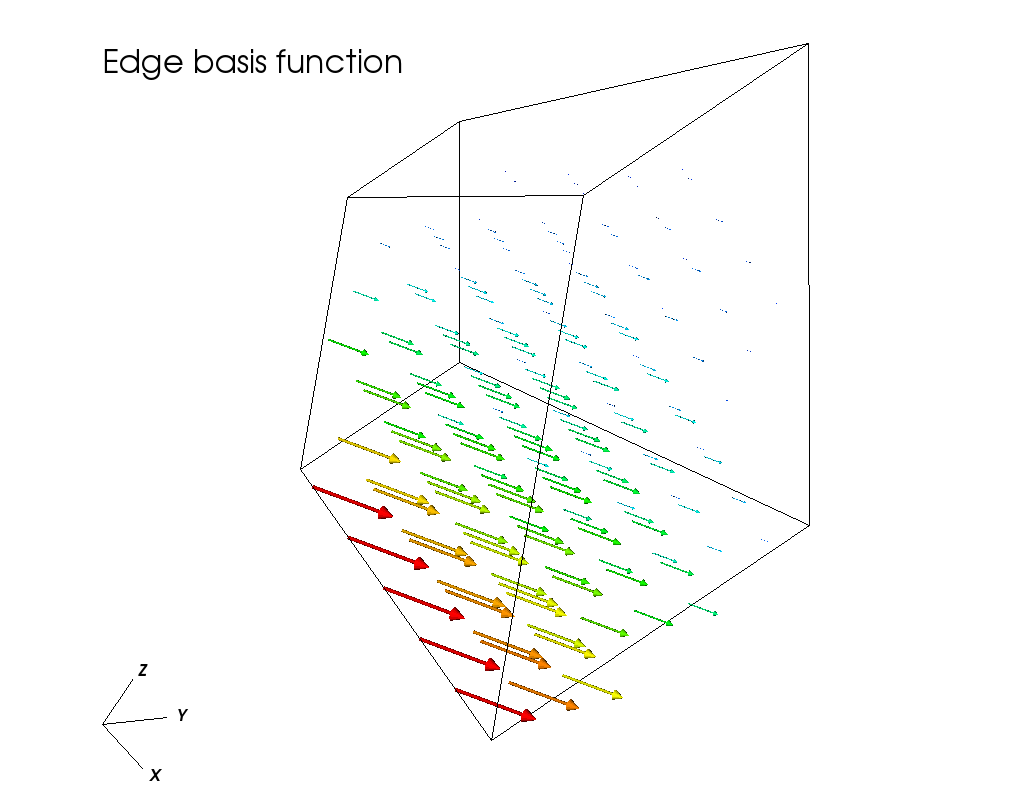
\includegraphics[width=50mm]{hexEdge.png} &                        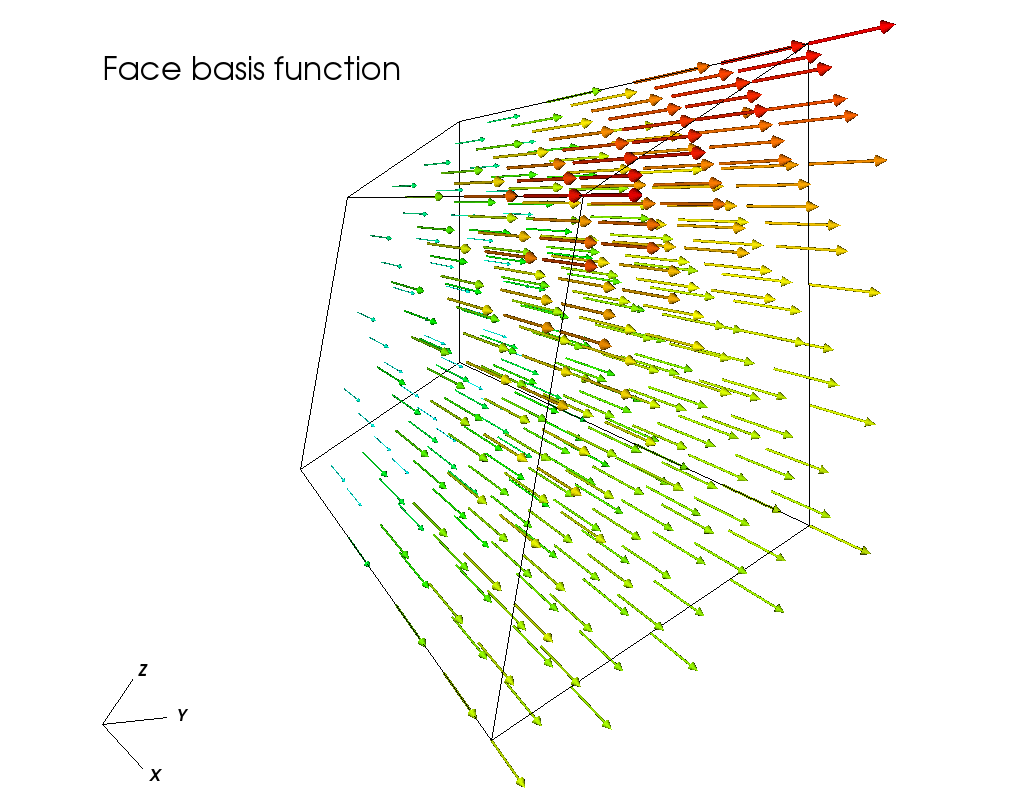
\includegraphics[width=50mm]{hexFace.png} \\
      {Edge basis is perpendicular } & {Face basis is tangent }  \\
      {to neighbouring edges} & {to neighbouring faces}
\end{tabular}

\end{frame}

\begin{frame}[t]
  \frametitle{Result 1: divergence-free field  $v = dz \wedge d\psi$}
  \begin{block}{Flux integral depends only on distance of endpoints to nearest grid node}
  \end{block}
  \begin{tabular}{c}
    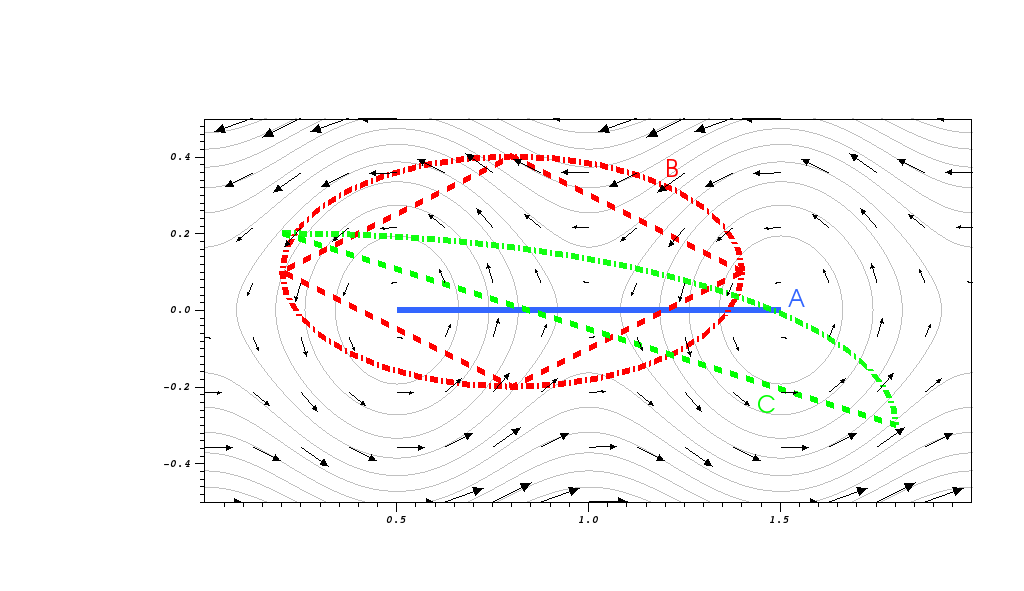
\includegraphics[width=.7\linewidth]{flow.png} \\
    Closed loop integral is exact!
  \end{tabular}
\end{frame}

\begin{frame}[t]
  \frametitle{Result 2: vector field $v = \frac{x dx + y dy}{2 \pi (x^2 + y^2)}$ with singularity}
  \begin{block}{Numerical loop integral A gives 0, B gives 1}
  \end{block}
  \begin{center}
    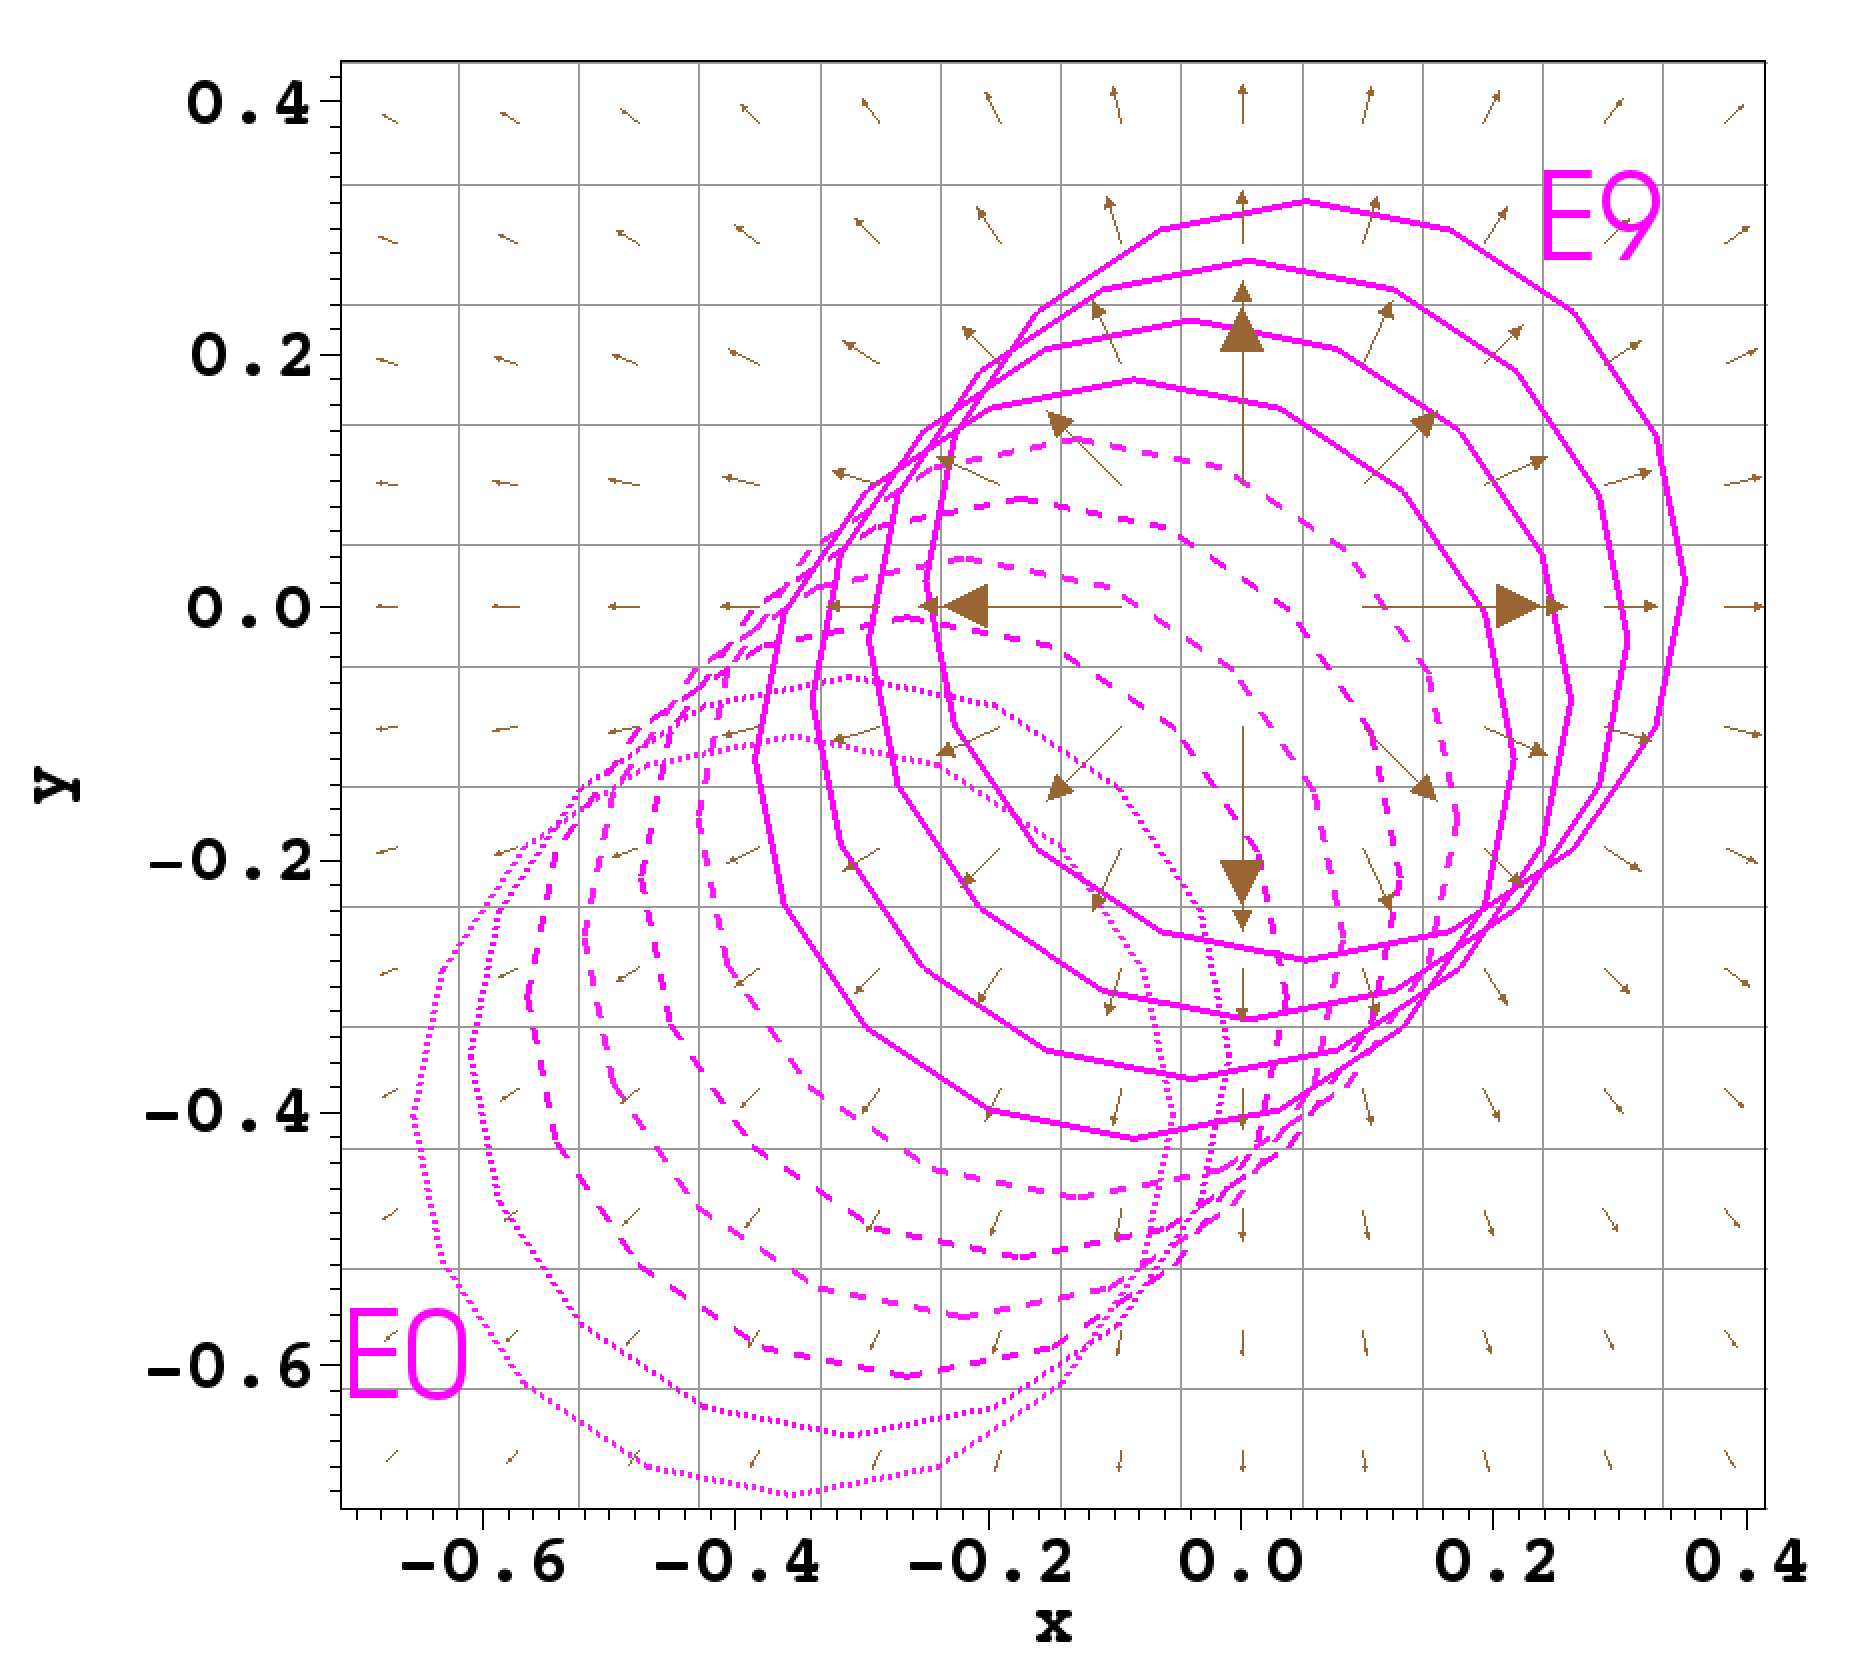
\includegraphics[width=.5\linewidth]{polar.png}
  \end{center}
\end{frame}

\begin{frame}[t]
  \frametitle{Result 3: flux on the cubed sphere $v = d\psi \wedge dr$}
  \begin{block}{Edge/face interpolation works for highly distorted cells}
  \end{block}
  
  \begin{tabular}{lr}
  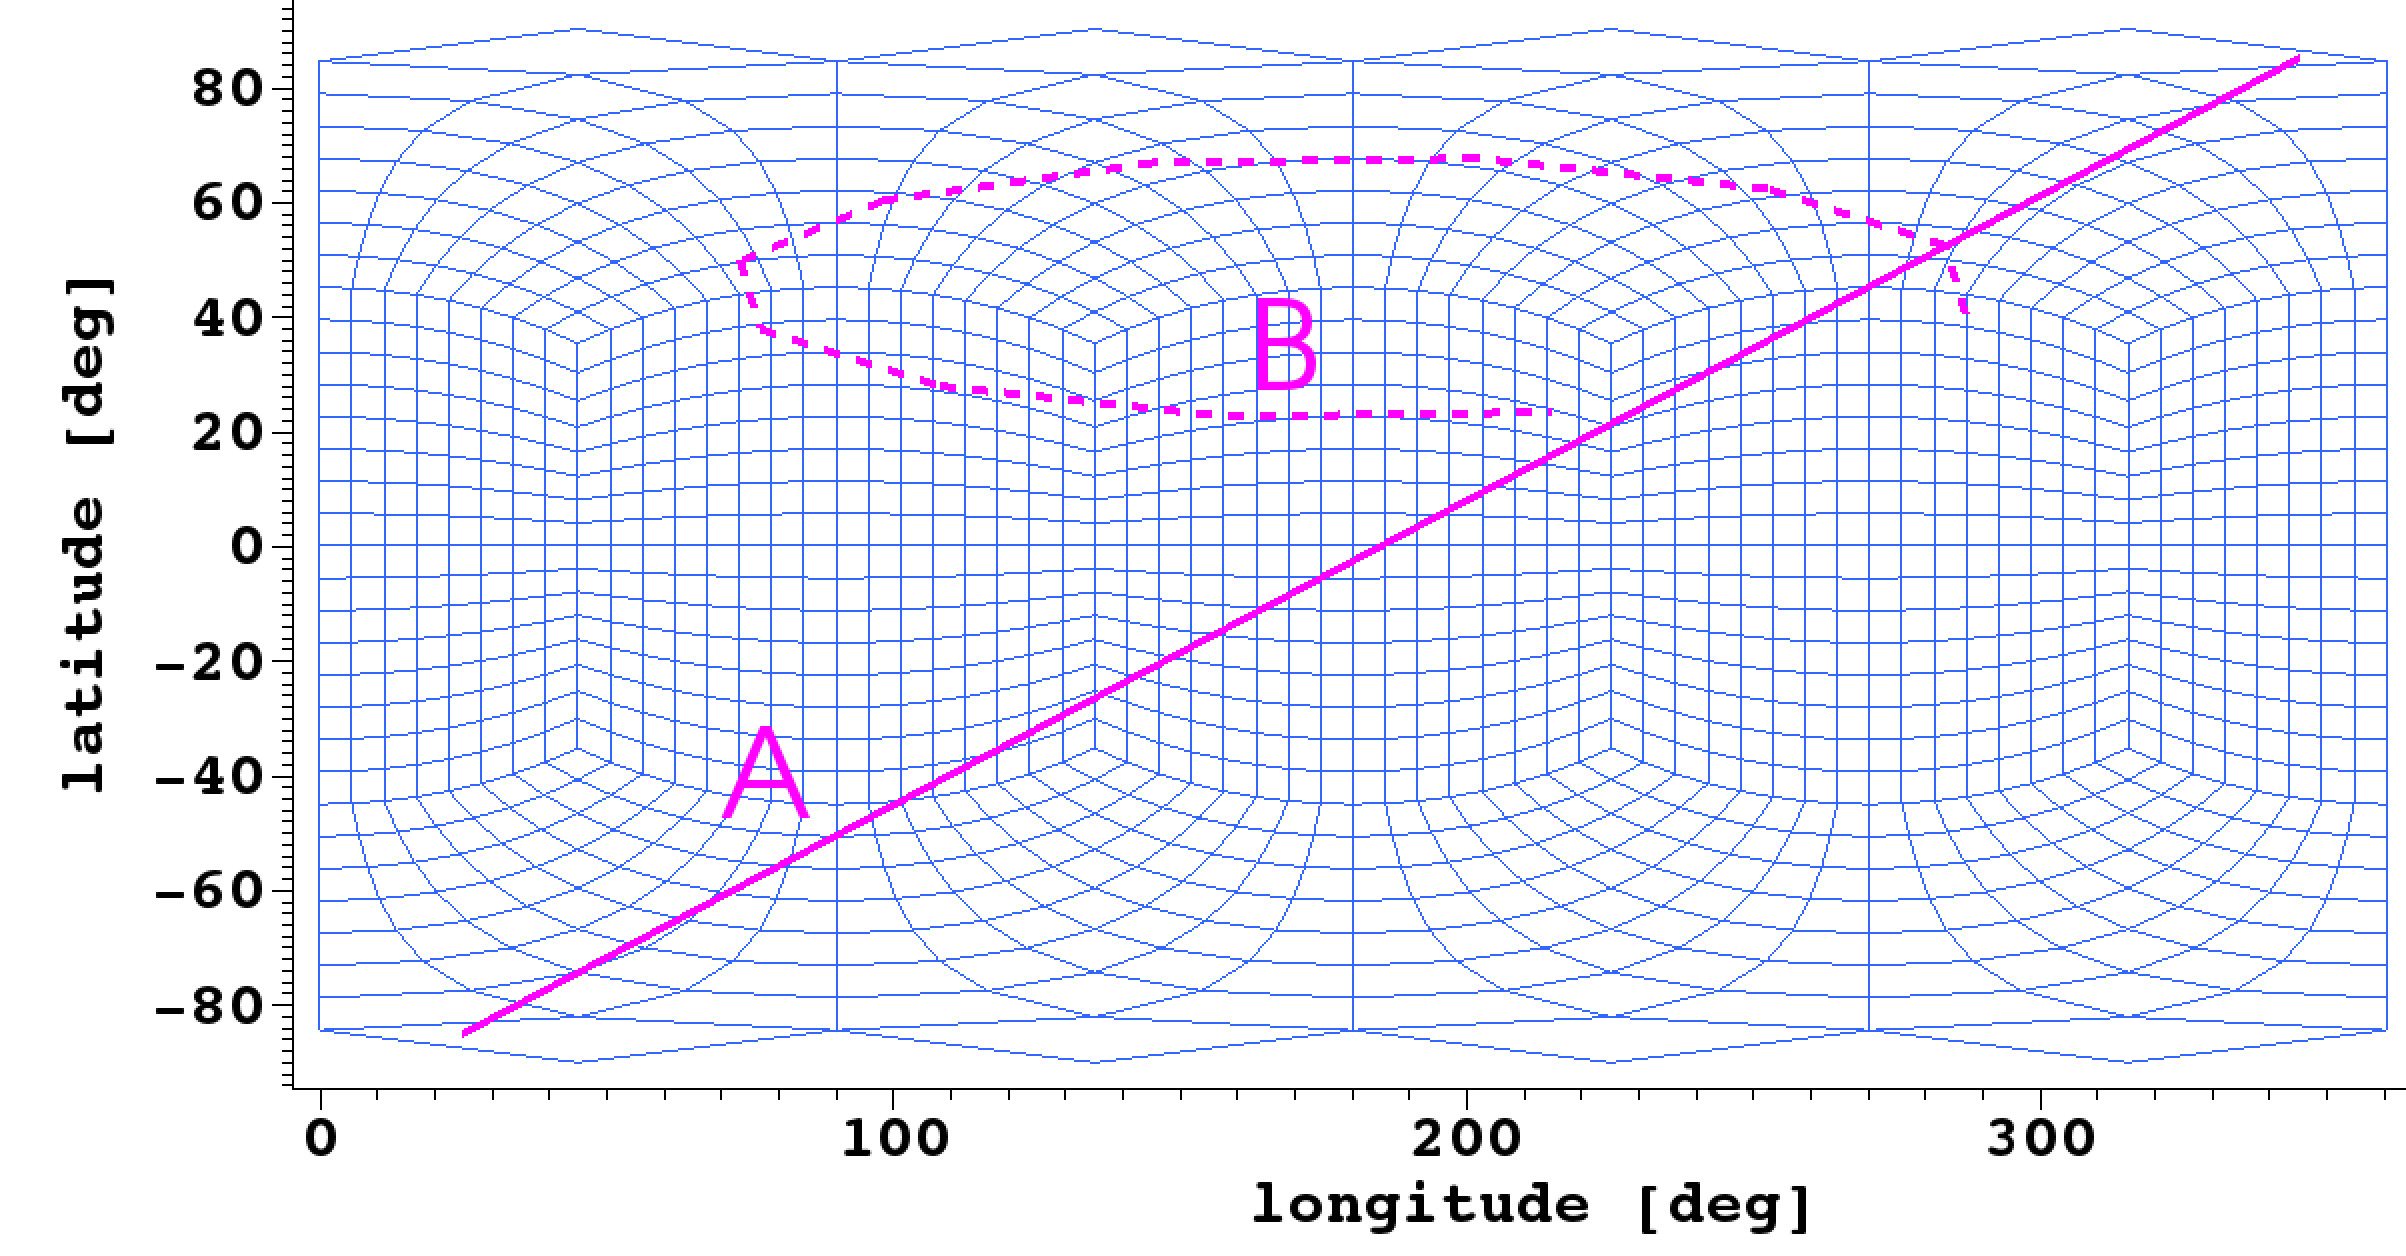
\includegraphics[width=75mm]{fluxOnCubedSphere.png} & 
  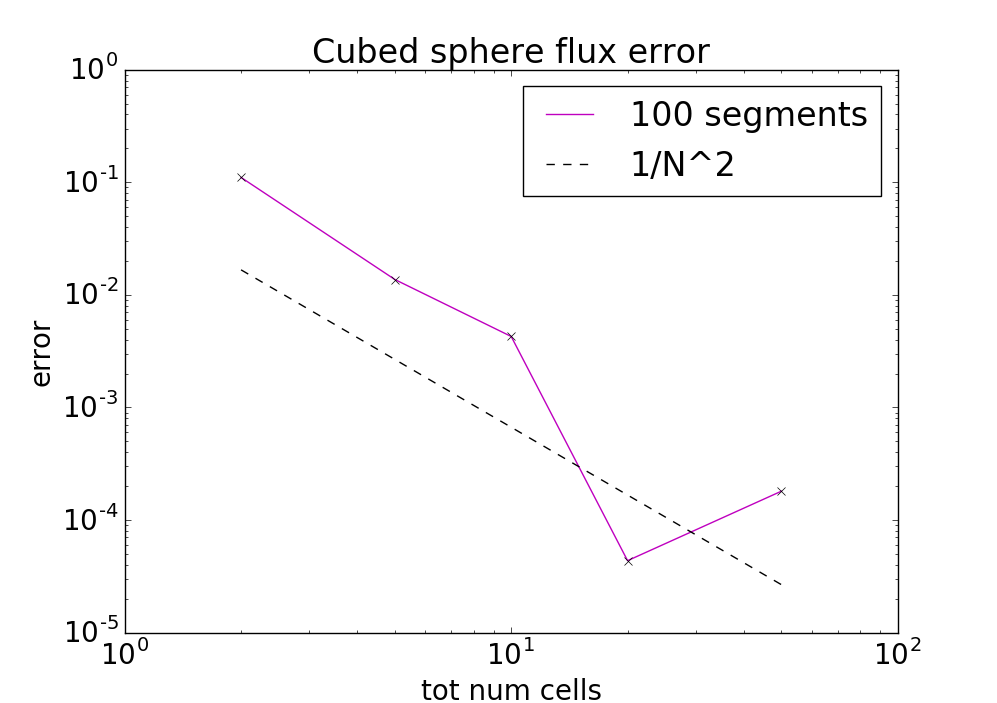
\includegraphics[width=60mm]{cubedSphereFluxError.png} \\
  {Integration path/surface} & {Error is $\sim 1/N^2$} 
  \end{tabular}
\end{frame}

\begin{frame}[t]
  \frametitle{Summary}
    \begin{block}{Different types of field $\leftrightarrow$ different staggerings}
      \begin{itemize}%[<+-| alert@+>]
	  \item nodal for scalar fields (e.g. temperature)
	  \item edge for vector fields (e.g. electric field, velocity)
	  \item face for pseudo-vector fields (e.g velocity)
	  \item cell for pseudo-scalar fields (e.g. density)
	  \item type of field $\rightarrow$ interpolation method
      \item field values set via cell, face and edge integrals (instead of vector field components)
    \end{itemize}
    \end{block}
    \begin{block}{Masking and partially valid cells?}
	 Ok if taking account of partial cell, faces, edges when setting cell, face and edge integrals. Done!
  \end{block}
\end{frame}

\begin{frame}[t]
  \frametitle{Summary (2)}
    \begin{block}{What about tetrahedra?}
      Similar approach except that the basis functions are Whitney's
    \end{block}
    \begin{block}{Higher order basis functions?}
    Initial work indicates that higher order basis functions can be used. These also satisfy the orthogonality condition $\int_i \phi_j = \delta_{ij}$
    on sub-cell edges, faces and cells. Quadratic elements effectively 
     split each cell into 8 sub-cells, each face into 4 sub-faces and each edge into 2 sub-edges. 
  \end{block}
    \begin{block}{The time is ripe to treat interpolation with same rigour as modelling}
    	``Mimetic Interpolation of Vector Fields on Arakawa C/D Grids'': https://journals.ametsoc.org/doi/10.1175/MWR-D-18-0146.1
  \end{block}
\end{frame}

\end{document} 